\documentclass{beamer}

\usepackage{beamerthemesplit}
\usepackage[utf8x]{inputenc}
\usepackage{pgf}
\usepackage{default}
\usepackage{url}
\usepackage{subfigure}
\usepackage{algorithmic} 
\usepackage{algorithm} 
\usepackage{amssymb}

\usetheme{Singapore}


%Define some commands for printing correct variables in math mode 
\newcommand{\av}{\textbf{a}}
\newcommand{\bv}{\textbf{b}}
\newcommand{\cv}{\textbf{c}}
\newcommand{\dv}{\textbf{d}}
\newcommand{\ev}{\textbf{e}}
\newcommand{\fv}{\textbf{f}}
\newcommand{\gv}{\textbf{g}}
\newcommand{\hv}{\textbf{h}}
\newcommand{\iv}{\textbf{i}}
\newcommand{\jv}{\textbf{j}}
\newcommand{\kv}{\textbf{k}}
\newcommand{\lv}{\textbf{l}}
\newcommand{\mv}{\textbf{m}}
\newcommand{\nv}{\textbf{n}}
\newcommand{\ov}{\textbf{o}}
\newcommand{\pv}{\textbf{p}}
\newcommand{\qv}{\textbf{q}}
\newcommand{\rv}{\textbf{r}}
\newcommand{\sv}{\textbf{s}}
\newcommand{\tv}{\textbf{t}}
\newcommand{\uv}{\textbf{u}}
\newcommand{\vv}{\textbf{v}}
\newcommand{\wv}{\textbf{w}}
\newcommand{\xv}{\textbf{x}}
\newcommand{\yv}{\textbf{y}}
\newcommand{\zv}{\textbf{z}}

\newcommand{\alphav}{\mbox{\boldmath$\alpha$}}
\newcommand{\betav}{\mbox{\boldmath$\beta$}}
\newcommand{\gammav}{\mbox{\boldmath$\gamma$}}
\newcommand{\xiv }{\mbox{\boldmath$\xi$}}
\newcommand{\muv}{\mbox{\boldmath$\mu$}}
\newcommand{\tauv}{\mbox{\boldmath$\tau$}}
\newcommand{\Omegam}{\mbox{\boldmath$\Omega$}}
\newcommand{\Lambdam}{\mbox{\boldmath$\Lambda$}}
\newcommand{\Sigmam}{\mbox{\boldmath$\Sigma$}}
\newcommand{\Gammam}{\mbox{\boldmath$\Gamma$}}
\newcommand{\Deltam}{\mbox{\boldmath$\Delta$}}
\newcommand{\Thetam}{\mbox{\boldmath$\Theta$}}
\newcommand{\Phim}{\mbox{\boldmath$\Phi$}}
\newcommand{\Pim}{\mbox{\boldmath$\Pi$}}

\newcommand{\diag}{\mbox{diag}}
\newcommand{\tr}{\mbox{tr}}
\newcommand{\card}{\mbox{card}}
\newcommand{\cov}{\mbox{cov}}
\newcommand{\sign}{\mbox{sign}}
\newcommand{\var}{\mbox{var}}
\newcommand{\st}{\mbox{s.t.}}
\newcommand{\rank}{\mbox{rank}}
\newcommand{\argmin}{\mbox{argmin}}
\newcommand{\argmax}{\mbox{argmax}}

\newcommand{\Am}{\textbf{A}}
\newcommand{\Bm}{\textbf{B}}
\newcommand{\Cm}{\textbf{C}}
\newcommand{\Dm}{\textbf{D}}
\newcommand{\Em}{\textbf{E}}
\newcommand{\Fm}{\textbf{F}}
\newcommand{\Gm}{\textbf{G}}
\newcommand{\Hm}{\textbf{H}}
\newcommand{\Imat}{\textbf{I}}
\newcommand{\Jm}{\textbf{J}}
\newcommand{\Km}{\textbf{K}}
\newcommand{\Lm}{\textbf{L}}
\newcommand{\Mm}{\textbf{M}}
\newcommand{\Nm}{\textbf{N}}
\newcommand{\Om}{\textbf{O}}
\newcommand{\Pm}{\textbf{P}}
\newcommand{\Qm}{\textbf{Q}}
\newcommand{\Rm}{\textbf{R}}
\newcommand{\Sm}{\textbf{S}}
\newcommand{\Tm}{\textbf{T}}
\newcommand{\Um}{\textbf{U}}
\newcommand{\Vm}{\textbf{V}}
\newcommand{\Wm}{\textbf{W}}
\newcommand{\Xm}{\textbf{X}}
\newcommand{\Ym}{\textbf{Y}}
\newcommand{\Zm}{\textbf{Z}}

%Use regular expression: (\[a-z])([^a-zA-Z])  -> \1v\2  to change old style macros 
\graphicspath{{./Figures/}}

\title{Statistics and the Analysis of Data\\ Lecture 1: Descriptive Statistics}
\author{Charanpal Dhanjal \\ \texttt{charanpal@gmail.com}} 
\institute{\'{E}cole des Ponts}
\date{\today}

\begin{document}

\frame{\titlepage}

\begin{frame}{Course Overview}
\begin{itemize}
\item Timetable 
\begin{itemize}
\item 8 lecture session of 2 hours
\item 4 TP sessions of 2 hours
\item 1 exam of 2 hours 
\end{itemize}
\item Overview
\begin{itemize} 
\item Descriptive Statistics - means, modes, histograms etc. 
\item Multivariate statistics - PCA, graphical models 
\item Multiple linear regression 
\end{itemize}
\end{itemize}
\end{frame}

\begin{frame}{Lecture Overview}
\begin{itemize} 
 \item Motivation 
\item What is statistics 
\item Statistical measures - means, medians, 
\item Graphical representations - histograms, QQPlots 
\end{itemize}
\end{frame}

\begin{frame}{Motivation} 
\begin{itemize} 
 \item Statistics underpins much of science and engineering in domains including: 
\begin{itemize} 
\item Meteorology, take measures to make predictions about the weather. Vital to provide early warnings for tornadoes, extreme weather at sea, gauge influence of human activity on global climate 
\item In drug design to measure the effectiveness of new drugs 
\item Marketing to develop a strategy to sell a product or service 
\end{itemize} 
\end{itemize}
\end{frame}

\begin{frame}{What is Statistics?}  
 \begin{itemize} 
\item Collection, study and interpretation of data 
\item Explore latent aspects of the data 
\item Statistics is the study of random variables  
 \end{itemize}
\end{frame}

\begin{frame}{Observed variables}
\begin{itemize} 
 \item Imagine that we have an experiment and see $n$ variables $x_1, \ldots, x_n$ (i.e. experiment is repeated $n$ times)
\begin{itemize} 
\item E.g. a vote, scientific experiment, roll of a die
\end{itemize}
\item We can say the values $x_1, \ldots, x_n$ are \emph{observations} of a random variable $X$ 
\item Two types of variables: 
\begin{itemize} 
 \item Discrete when $X$ is chosen from a finite set e.g. A die has 6 values $1-6$ 
\item Continuous $X$ is infinite within a certain range e.g. all real numbers in the range $[0, 10]$
\end{itemize}
\end{itemize}
\end{frame}

\begin{frame}{Histogram of discrete variables I} 
\begin{itemize} 
 \item A histogram represents the distribution of values in a set of observations
\item Can call it a function $h: \mathbb{R} \mapsto \mathbb{N}$ which is the frequency of each observation 
\begin{displaymath} 
 h(x) = \sum_{i=1}^n \mathcal{I}(x_i = x)
\end{displaymath}
\item Or, a normalised histogram
\begin{displaymath} 
  h(x) = \frac{1}{n}\sum_{i=1}^n \mathcal{I}(x_i = x)
\end{displaymath}
\end{itemize}
\end{frame}

\begin{frame}{Histogram of discrete variables II}
\begin{itemize}
 \item E.g. roll a die 100 times 
\end{itemize}
\begin{figure}[htp]
\mbox{
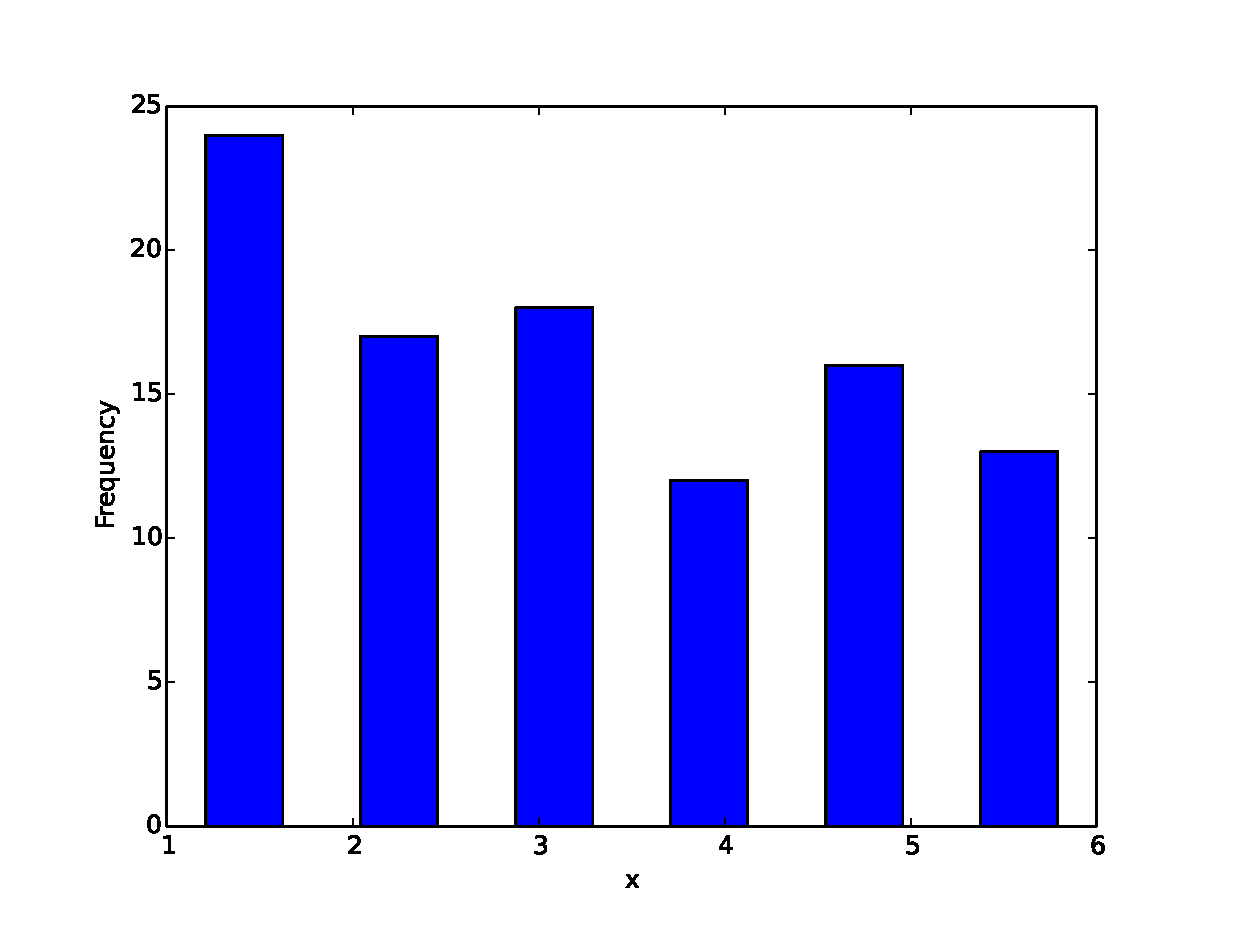
\includegraphics[width=0.5\linewidth]{DiscreteHist.eps}
}
\end{figure}
\end{frame}

\begin{frame}{Histograms of Continuous Variables I}  
 \begin{itemize} 
  \item First partition input space into a series of \emph{bins} $I_0, I_1, \ldots, I_k$ 
  \item Then count the number of elements in each bin: $n_j = \sum_{x_i} x_i \in I_j$
  \item Can normalise to compute a density : 
  \begin{displaymath} 
    h(y) = \frac{n_j}{n |I_j|} \quad \forall y \in I_j
  \end{displaymath}
 \end{itemize}
\end{frame}

\begin{frame}{Histograms of Continuous Variables II}  
\begin{itemize}
 \item E.g. the normal distribution sampled 100 times 
\end{itemize}
\begin{figure}[htp]
\mbox{
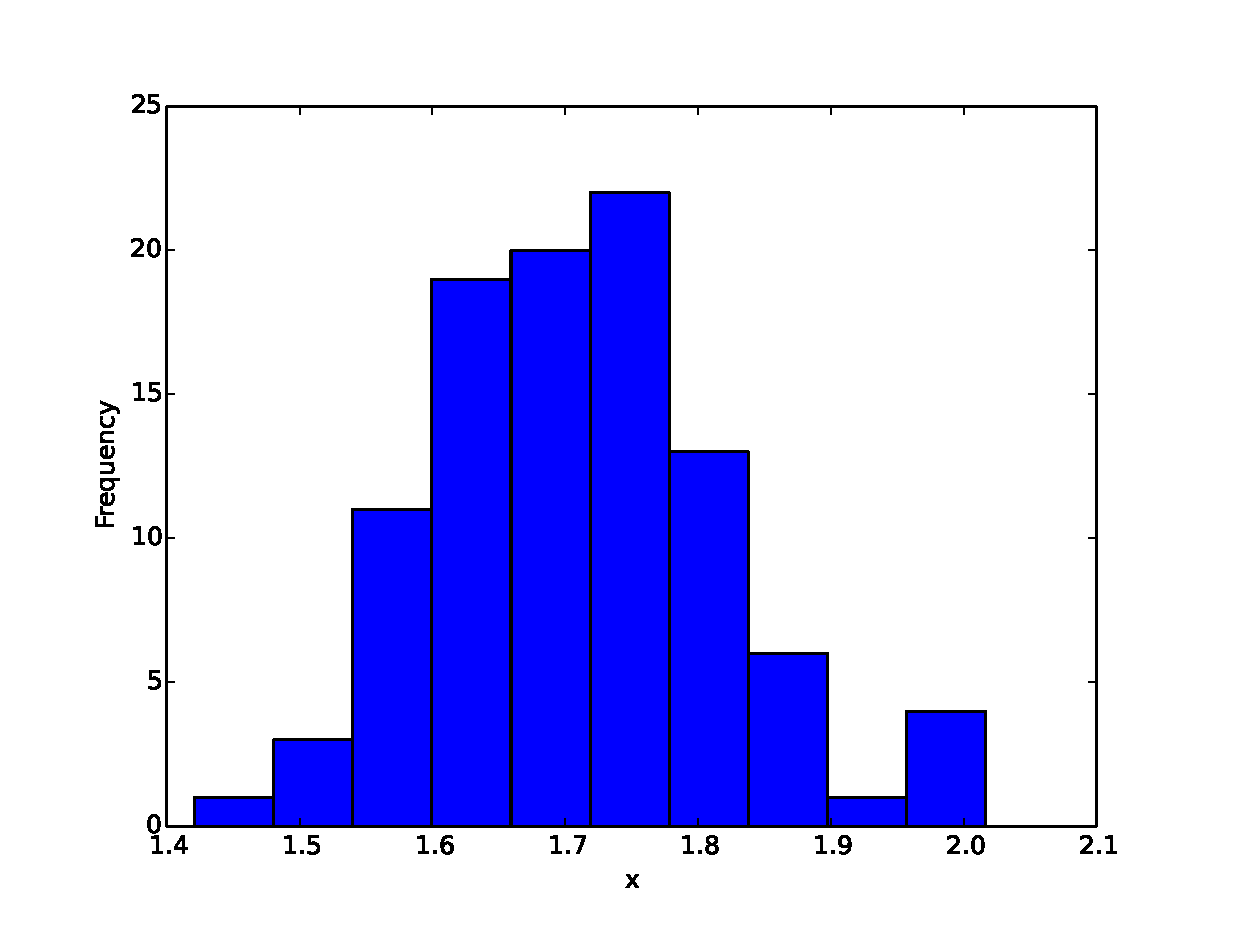
\includegraphics[width=0.5\linewidth]{ContinuousHist.eps}
}
\end{figure} 
\end{frame}

\begin{frame}{Cumulative Distribution Function}  
\begin{itemize} 
 \item Another representation of the distribution of values 
\item The cumulative distribution function is the proportion of values less than $x$
\begin{displaymath}
 F(x) = \frac{1}{n}\sum_{i=1}^n I(x_i \leq x)
\end{displaymath}
\item The definition is the same for discrete and continuous variables 
\end{itemize}
 \begin{figure}[htp]
\mbox{
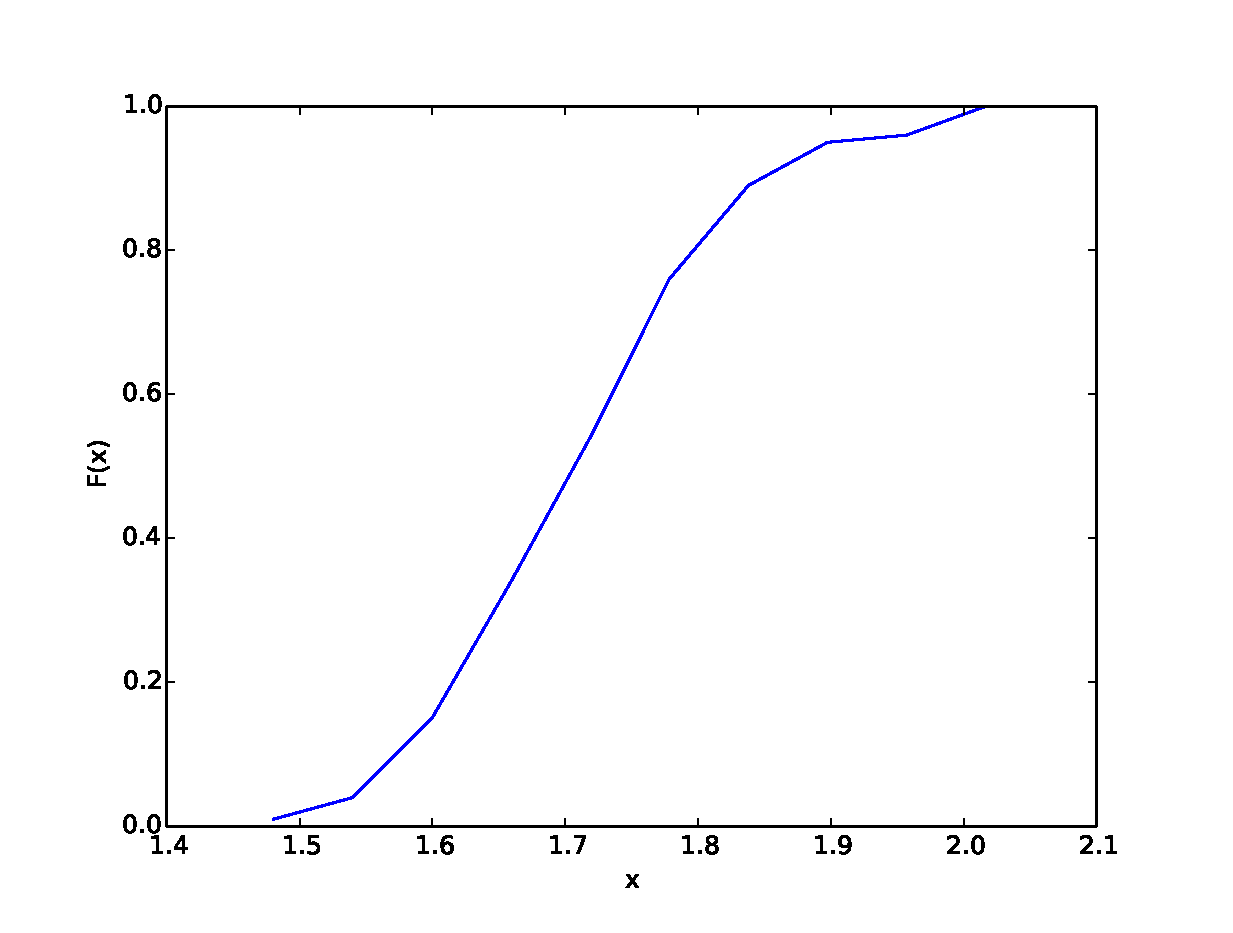
\includegraphics[width=0.5\linewidth]{ContinuousCDF.eps}
}
\end{figure} 
\end{frame}

\begin{frame}{Measures of Average}
\begin{itemize} 
 \item Look at statistics to summarise data $x_1, \ldots x_n$
  \item The \emph{mean} is defined as 
  \begin{displaymath}
   \bar{x} = \frac{1}{n}\sum_{i=1}^n x_i
  \end{displaymath}
\item The \emph{median} is the value such that $med(x)$ separates the higher half of the data from the lower half 
\item The \emph{mode} $mod(x)$ is the most common value  
\end{itemize}
\end{frame}

\begin{frame}{Computing averages} 
 \begin{itemize} 
  \item Example, tossing a die: 
\begin{table}
  \begin{tabular}{l | l l l l l l }
\hline 
  Outcome & 1 & 2 & 3 & 4 & 5 & 6 \\ 
  Frequency & 3 & 1 & 4 & 5 & 5 & 2 \\
\hline 
  \end{tabular} 
\end{table}
  \item Mean is 3.7 
  \item Median is 4 
  \item Mode is 4 or 5 
 \end{itemize}
\end{frame}

\begin{frame}{Dispersion}  
\begin{itemize} 
 \item Gauge the variation in the values 
\begin{itemize} 
\item The \emph{variance} is the mean square difference with the mean 
\begin{displaymath} 
 var(x) = \frac{1}{n}\sum_{i=1}^n (x_i - \bar{x})^2
\end{displaymath}
 \item The \emph{standard deviation} is the root of the variance $std(x) = \sqrt{var(x)}$. 
\item Analogously the \emph{mean absolute deviation} is 
\begin{displaymath} 
  mad(x) = \frac{1}{n}\sum_{i=1}^n |x_i - med(x)|
\end{displaymath}
\end{itemize}
\end{itemize}
\end{frame}

\begin{frame}{Interquartile range} 
 \begin{itemize} 
  \item Let $Q1$ be the median value less than $med(x)$ 
  \item Let $Q3$ be the median value greater than $med(x)$
  \item The \emph{interquartile range} is $Q3 - Q1$ 
 \end{itemize}
\end{frame}

\begin{frame}{Exercises}  
 
\end{frame}


\end{document}
